\documentclass{scrartcl}
\usepackage[T1]{fontenc}

% u/ masukin gambar
\usepackage{graphicx}

% u/ bikin ornament

% u/ mengatur margin kertas
\usepackage{geometry}
\geometry{
	a4paper,
	left=3.5cm,
	right=2.5cm,
	bottom=2.5cm,
	top=3cm
}

% u/ referensi
\usepackage{hyperref}

% u/ bikin tabel
\usepackage{tabu}
\usepackage{booktabs}

% u/ masukin source code
\usepackage{minted}
\usemintedstyle{vs}
\setminted[]{
	breaklines=true,
	tabsize=2,
	autogobble=true
}

% Content -> Daftar Isi
\renewcommand{\contentsname}{Daftar Isi}

\begin{document}

% kop judul handout
\begin{center}
\begin{tabu} to \linewidth {X[c]}
	\toprule
	\\
	\LARGE{\textbf{Handout Praktikum Mobile Application}} \\
	\\
	\large{Topik 1 -- Activity dan Intent} \\
	\\
	\bottomrule
\end{tabu}
\end{center}

\tableofcontents


\section{Tujuan}
\begin{enumerate}
	\item Mahasiswa dapat memahami siklus hidup \textit{activity}
	\item Mahasiswa dapat menentukan gaya dan tema \textit{activity}
	\item Mahasiswa dapat menampilkan \textit{activity} sebagai jendela dialog
	\item Mahasiswa dapat memahami konsep \textit{intent}
\end{enumerate}

\section{Komponen/Peralatan}
\begin{itemize}
	\item PC/laptop
	\item Android Studio
\end{itemize}

\section{Dasar Teori}

Aplikasi Android memiliki banyak komponen, salah empatnya adalah \textit{activity}, \textit{service}, \textit{broadcast receiver}, dan \textit{content provider}. Hari ini kita khusus mempelajari \textit{activity}.

\textit{Activity} adalah komponen UI paling utama. Setidaknya dalam satu aplikasi terdapat satu buah \textit{activity}. Di dalamnya bisa kamu isi dengan \textit{View} dan \textit{ViewGroup}. Contoh \textit{View} adalah \texttt{TextView} yang berfungsi untuk menampung \textit{string}. Selain itu ada pula \texttt{Button} yang berfungsi layaknya \textit{push-button} dalam dunia nyata. \textit{ViewGroup} berfungsi untuk memberikan tata letak \textit{View}. Dalam praktikum ini, kita tidak akan membahas detail mengenai \textit{user interface}.

Setiap \textit{activity} mempunyai siklus hidup-nya masing-masing. Berikut ini adalah diagram \textit{state}-nya.

\begin{figure}[htbp]
	\centering
	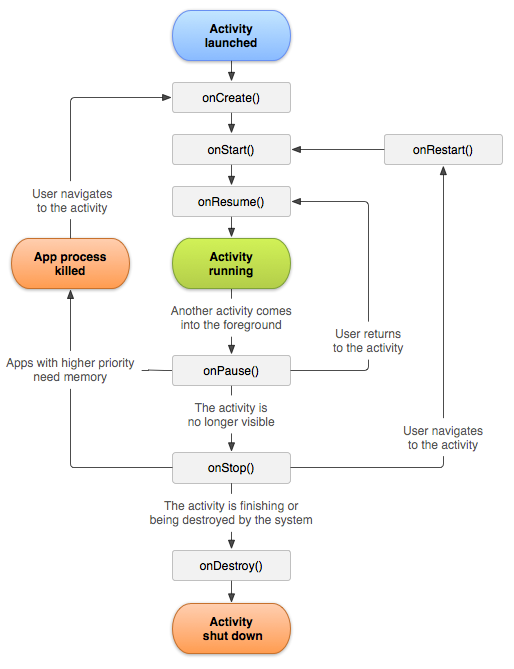
\includegraphics[width=0.7\linewidth]{screenshot001}
	\caption{Siklus Hidup \textit{Activity}}
	\label{fig:screenshot001}
\end{figure}

Dalam percobaan 4.1 kalian akan mencoba memperhatikan siklus hidup \textit{activity}.

Dalam satu aplikasi biasanya ada banyak \textit{activity}. Jika kasusnya demikian, mungkin kamu harus menggunakan \texttt{intent} untuk menghubungkan antar \textit{activity}.

Untuk keterangan lebih lanjut silahkan baca \textit{website} resmi Android.


\section{Langkah Praktikum}

\subsection{Memahami Siklus Hidup \texttt{Activity}}

\begin{enumerate}
	\item Buat proyek baru dengan ketentuan sebagai berikut.
	\begin{itemize}
		\item Nama aplikasi $\rightarrow$ \textbf{Activity101}
		\item Pilih \textit{template} activity $\rightarrow$ \textbf{Empty Activity}
		\item Nama activity $\rightarrow$ \textbf{Activity101Activity}
	\end{itemize}

	\item Buka file \texttt{Activity101Activity.java} lalu \textit{copy-paste} listing di bawah ini.
	
	\begin{minted}{java}
	package com.example.activity101;
	
	import android.support.v7.app.AppCompatActivity;
	import android.os.Bundle;
	import android.util.Log;
	
	public class Activity101Activity extends AppCompatActivity {
	
		String tag = "Lifecycle Step";
		
		@Override
		protected void onCreate(Bundle savedInstanceState) {
			super.onCreate(savedInstanceState);
			setContentView(R.layout.activity_activity101);
			Log.d(tag, "In the OnCreate() event");
		}
		
		public void onStart()  {
			super.onStart();
			Log.d(tag, "In the onStart() event");
		}
	
		public void onRestart() {
			super.onRestart();
			Log.d(tag, "In the onRestart() event");
		}
	
		public void onResume() {
			super.onResume();
			Log.d(tag, "In the onResume() event");
		}
	
		public void onPause() {
			super.onPause();
			Log.d(tag, "In the onPause() event");
		}
		
		public void onStop() {
			super.onStop();
			Log.d(tag, "In the onStop() event");
		}
	
		public void onDestroy() {
			super.onDestroy();
			Log.d(tag, "In the onDestroy() event");
		}
	}
	\end{minted}

	\item Tekan \texttt{Shift + F9} (atau pilih \texttt{Run > Debug}) untuk men-\textit{debug} aplikasi. Pilih salah satu Android Virtual Device yang kalian inginkan.
	
	\item Ketika \texttt{Activity} pertama kali berjalan, kamu akan melihat baris log pada konsol logcat yang mirip seperti berikut ini.

	\begin{minted}{bash}
	06-04 17:42:48.344 21251-21251/com.example.activity101 D/Lifecycle Step: In the OnCreate() event
	06-04 17:42:48.344 21251-21251/com.example.activity101 D/Lifecycle Step: In the onStart() event
	06-04 17:42:48.345 21251-21251/com.example.activity101 D/Lifecycle Step: In the onResume() event
	\end{minted}

	\item Tekan tombol Back pada emulator, lalu perhatikan konsol logcat. Terdapat baris log seperti berikut.
	
	\begin{minted}{bash}
	06-04 17:43:17.148 21251-21251/com.example.activity101 D/Lifecycle Step: In the onPause() event
	06-04 17:43:17.610 21251-21251/com.example.activity101 D/Lifecycle Step: In the onStop() event
	06-04 17:43:17.610 21251-21251/com.example.activity101 D/Lifecycle Step: In the onDestroy() event
	
	\end{minted}
	
	\item	Tekan tombol Home pada emulator, jalankan kembali aplikasi Activity101, lalu perhatikan konsol logcat. Terdapat baris log seperti berikut.
	
	\begin{minted}{bash}
	06-04 17:44:20.841 21251-21251/com.example.activity101 D/Lifecycle Step: In the OnCreate() event
	06-04 17:44:20.842 21251-21251/com.example.activity101 D/Lifecycle Step: In the onStart() event
	06-04 17:44:20.844 21251-21251/com.example.activity101 D/Lifecycle Step: In the onResume() event
	\end{minted}
	
	\item Tekan tombol Home pada emulator, jalankan aplikasi Phone, lalu perhatikan konsol logcat. Terdapat baris log seperti berikut.
	
	\begin{minted}{bash}
	06-04 17:44:57.703 21251-21251/com.example.activity101 D/Lifecycle Step: In the onPause() event
	06-04 17:44:57.748 21251-21251/com.example.activity101 D/Lifecycle Step: In the onStop() event
	\end{minted}
	
	\item Perhatikan bahwa \textit{event} \texttt{onDestroy()} tidak terpanggil. Terakhir, tekan tombol Back pada emulator, jalankan aplikasi Activity101, lalu perhatikan konsol logcat. Terdapat baris log seperti berikut.
	
	\begin{minted}{bash}
	06-04 17:46:51.928 21251-21251/com.example.activity101 D/Lifecycle Step: In the onRestart() event
	06-04 17:46:51.928 21251-21251/com.example.activity101 D/Lifecycle Step: In the onStart() event
	06-04 17:46:51.929 21251-21251/com.example.activity101 D/Lifecycle Step: In the onResume() event
	\end{minted}

\end{enumerate}

\subsection{Menampilkan Jendela Dialog Menggunakan \texttt{Activity}}

\begin{enumerate}
	\item Buat proyek baru dengan ketentuan berikut ini.
	\begin{itemize}
		\item Nama aplikasi $\rightarrow$ \textbf{Dialog}
		\item Pilih \textit{template} activity $\rightarrow$ \textbf{Basic Activity}.
		\item Nama \textit{activity} $\rightarrow$ \textbf{DialogActivity}.
	\end{itemize}
	
	\item Buka file \texttt{AndroidManifest.xml}, lalu \textit{copy-paste} listing berikut ini.
	
	\begin{minted}{xml}
	<?xml version="1.0" encoding="utf-8"?>
	<manifest xmlns:android="http://schemas.android.com/apk/res/android"
		package="com.example.dialog" >
		
		<application
			android:allowBackup="true"
			android:icon="@mipmap/ic_launcher"
			android:label="@string/app_name"
			android:roundIcon="@mipmap/ic_launcher_round"
			android:supportsRtl="true"
			android:theme="@style/AppTheme" >
			<activity
				android:name=".DialogActivity"
				android:label="@string/app_name"
				android:theme="@style/Theme.AppCompat.Dialog" >
				<intent-filter>
					<action android:name="android.intent.action.MAIN" />
					
					<category android:name="android.intent.category.LAUNCHER" />
				</intent-filter>
			</activity>
		</application>
	
	</manifest>
	\end{minted}
	
	\item Tekan \texttt{Shift+F9} (atau pilih \texttt{Run > Debug}) untuk men-\textit{debug} aplikasi. Pilih salah satu Android Virtual Devices yang kalian inginkan. Hasil akhir ditunjukkan pada Figure \ref{fig:screenshot_1496826673}.
	
	\begin{figure}[htbp]
		\centering
		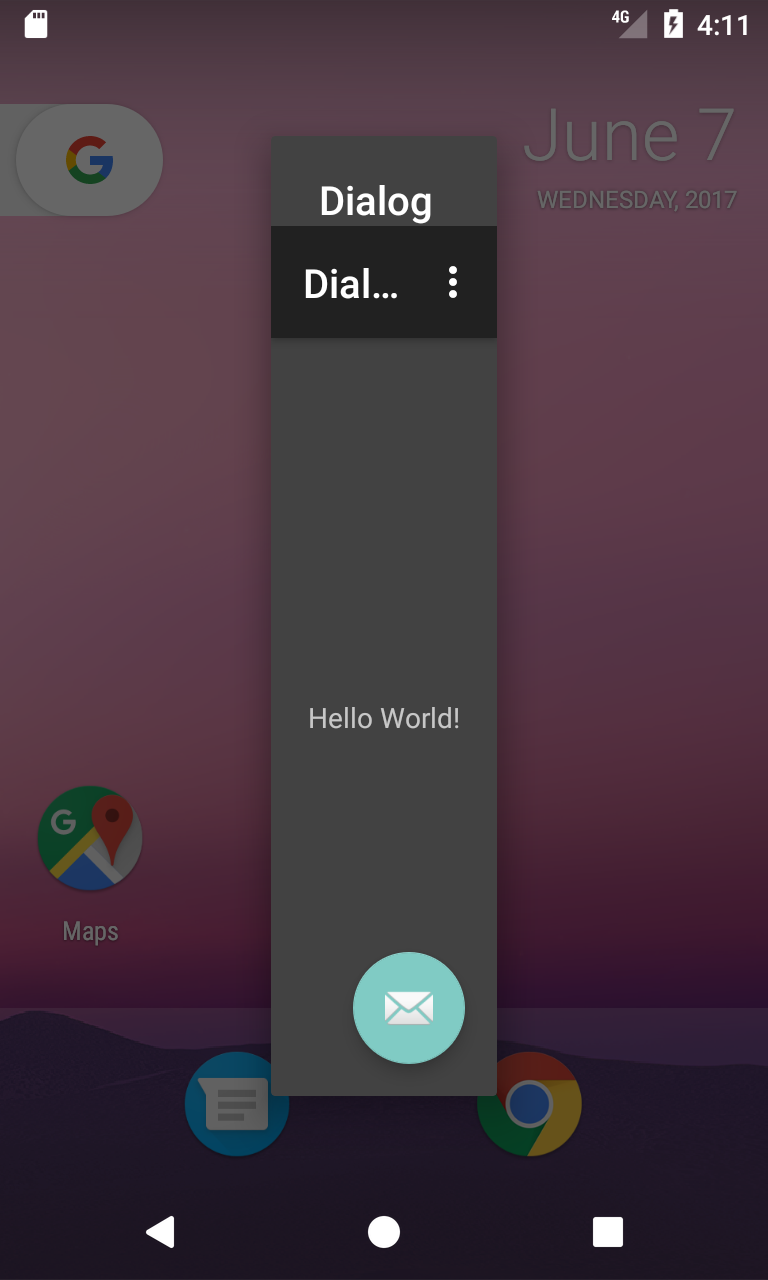
\includegraphics[width=0.5\linewidth]{Screenshot_1496826673}
		\caption{Hasil Akhir}
		\label{fig:screenshot_1496826673}
	\end{figure}
	
\end{enumerate}

\subsection{Menampilkan Dialog Perkembangan}

\begin{enumerate}
	\item Gunakan kembali proyek \textbf{Activity101}.
	
	\item Buka file \texttt{AndroidManifest.xml}, lalu \textit{copy-paste} listing berikut ini.
	
	\begin{minted}{xml}
	<?xml version="1.0" encoding="utf-8"?>
	<manifest xmlns:android="http://schemas.android.com/apk/res/android"
		package="com.example.activity101">
		
		<application
			android:allowBackup="true"
			android:icon="@mipmap/ic_launcher"
			android:label="@string/app_name"
			android:roundIcon="@mipmap/ic_launcher_round"
			android:supportsRtl="true"
			android:theme="@android:style/Theme.Material">
			<activity android:name=".Activity101Activity">
				<intent-filter>
					<action android:name="android.intent.action.MAIN" />
					
					<category android:name="android.intent.category.LAUNCHER" />
				</intent-filter>
			</activity>
		</application>
		
	</manifest>
	\end{minted}
	
	\item Buka file \texttt{Activity101Activity.java}, lalu \textit{copy-paste} listing berikut ini.
	
	\begin{minted}{java}
	package com.example.activity101;
	
	import android.app.Activity;
	import android.app.ProgressDialog;
	import android.os.Bundle;
	import android.os.CountDownTimer;
	
	public class Activity101Activity extends Activity {
	
		ProgressDialog progressDialog;
		
		@Override
		protected void onCreate(Bundle savedInstanceState) {
			super.onCreate(savedInstanceState);
			setContentView(R.layout.activity_activity101);
		}
		
		public void onStart()
		{
			super.onStart();
			progressDialog = ProgressDialog.show(this, "Please Wait", "Processing...", true);
			CountDownTimer timer = new CountDownTimer(3000, 1000) {
				@Override
				public void onTick(long millisUntilFinished) {
				
				}
				
				@Override
					public void onFinish() {
					progressDialog.dismiss();
				}
			}.start();
		}
	}
	
	\end{minted}
	
	\item Tekan \texttt{Shift+F9} (atau pilih \texttt{Run > Debug}) untuk men-\textit{debug} aplikasi. Pilih salah satu Android Virtual Devices yang kalian inginkan. Hasil akhir ditunjukkan pada Figure \ref{fig:screenshot_1496827169} dan Figure \ref{fig:screenshot_1496834779}.
	
	\begin{figure}[htbp]
	\begin{minipage}{.5\textwidth}
		\centering
		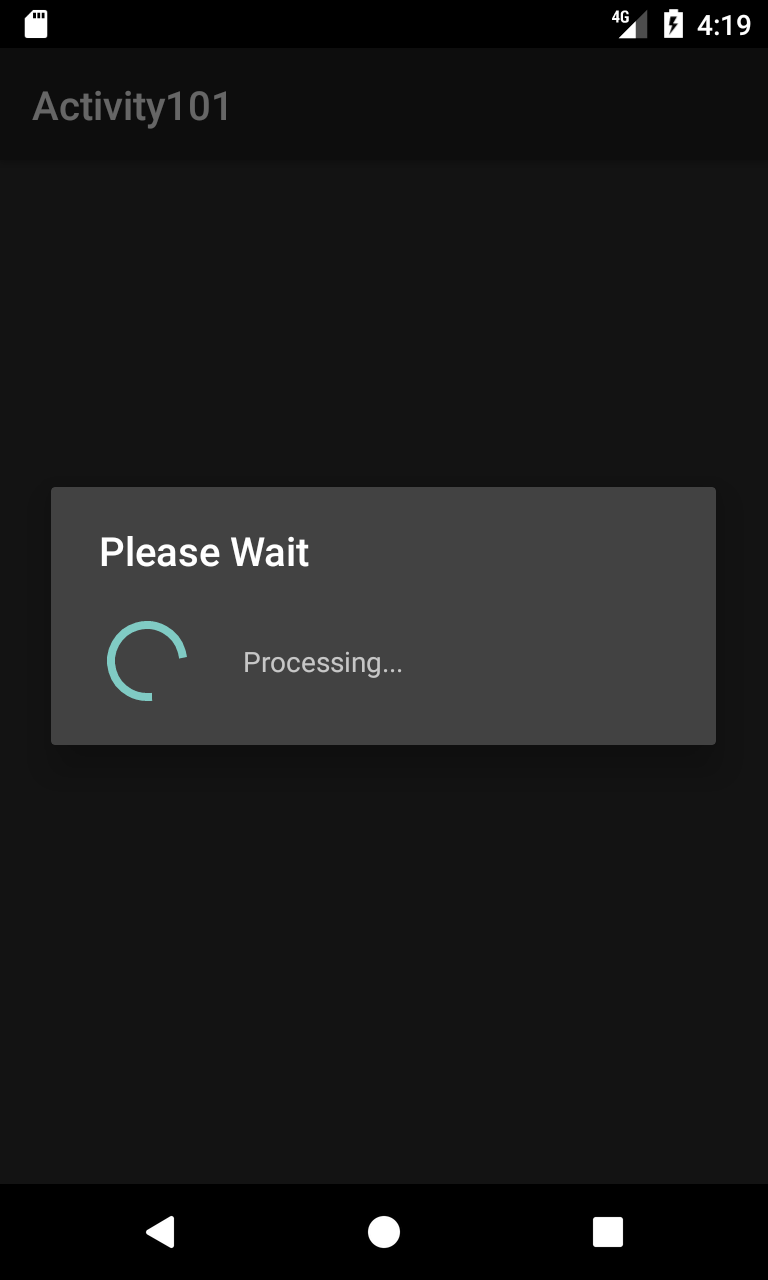
\includegraphics[width=0.7\linewidth]{Screenshot_1496827169}
		\caption{Hasil Akhir (1)}
		\label{fig:screenshot_1496827169}
	\end{minipage}
	\begin{minipage}{.5\textwidth}
		\centering
		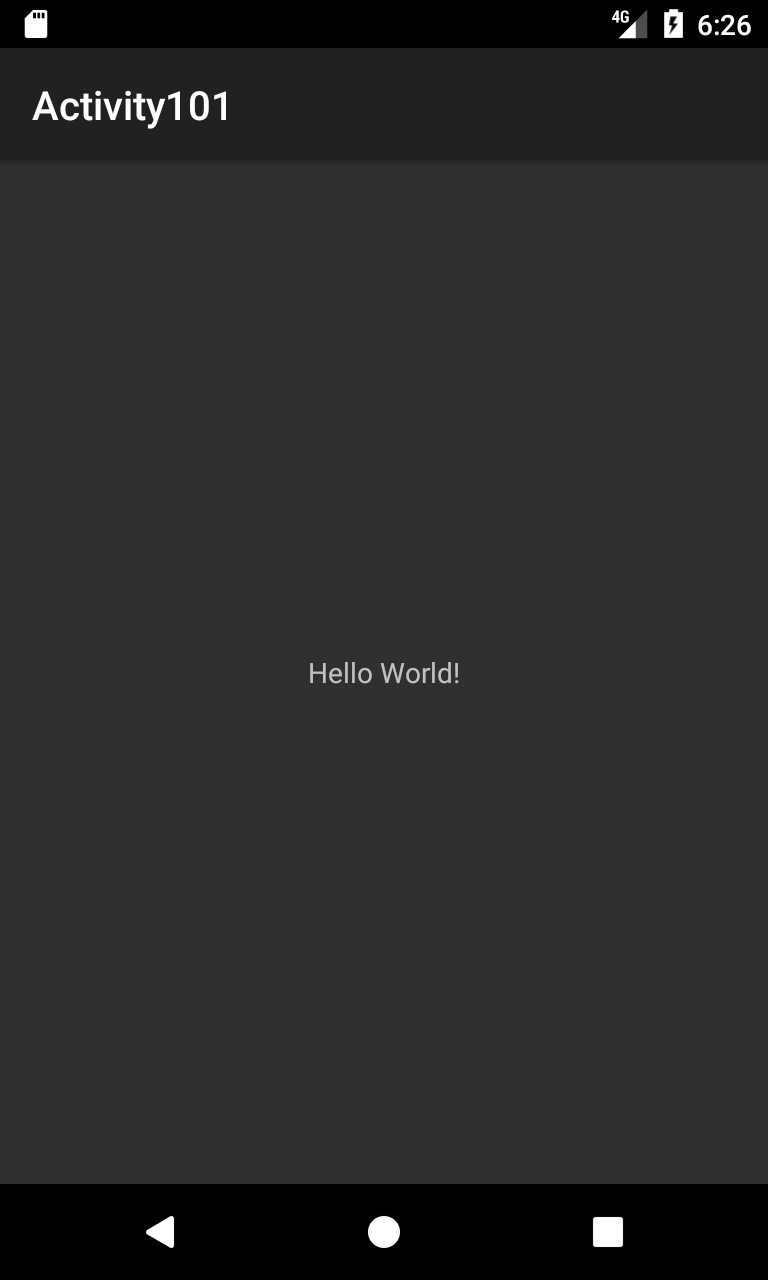
\includegraphics[width=0.7\linewidth]{Screenshot_1496834779}
		\caption{Hasil Akhir (2)}
		\label{fig:screenshot_1496834779}
	\end{minipage}
	\end{figure}

\end{enumerate}

\subsection{Menghubungkan Antar \texttt{Activity} Menggunakan \texttt{Intent}}

\begin{enumerate}
	\item Buat proyek baru dengan ketentuan berikut ini.
	\begin{itemize}
		\item Nama aplikasi $\rightarrow$ \textbf{UsingIntent}
		\item Pilih \textit{template} activity $\rightarrow$ \textbf{Empty Activity}.
	\end{itemize}
	\item Pilih \texttt{File > New > Activity > Empty Activity}. \texttt{Activity} yang baru tersebut diberi nama \textbf{SecondActivity}.
	\item Buka \texttt{AndroidManifest.xml} lalu \textit{copy-paste} listing berikut ini
	\begin{minted}{xml}
	<?xml version="1.0" encoding="utf-8"?>
	<manifest xmlns:android="http://schemas.android.com/apk/res/android"
		package="com.example.usingintent">
		
		<application
			android:allowBackup="true"
			android:icon="@mipmap/ic_launcher"
			android:label="@string/app_name"
			android:roundIcon="@mipmap/ic_launcher_round"
			android:supportsRtl="true"
			android:theme="@style/AppTheme">
			<activity android:name=".MainActivity">
				<intent-filter>
					<action android:name="android.intent.action.MAIN" />
					<category android:name="android.intent.category.LAUNCHER" />
				</intent-filter>
			</activity>
			<activity android:name=".SecondActivity">
				<intent-filter>
					<action android:name="com.example.usingintent.SecondActivity" />
					<category android:name="android.intent.category.DEFAULT" />
				</intent-filter>
			</activity>
		</application>
	
	</manifest>
	\end{minted}
	\item Buka \texttt{activity\_main.xml}, lalu \textit{copy-paste} listing berikut ini.
	\begin{minted}{xml}
	<?xml version="1.0" encoding="utf-8"?>
	<android.support.constraint.ConstraintLayout xmlns:android="http://schemas.android.com/apk/res/android"
		xmlns:app="http://schemas.android.com/apk/res-auto"
		xmlns:tools="http://schemas.android.com/tools"
		android:layout_width="match_parent"
		android:layout_height="match_parent"
		tools:context="com.example.usingintent.MainActivity">
		
		<TextView
			android:layout_width="wrap_content"
			android:layout_height="wrap_content"
			android:text="Main Activity!"
			android:id="@+id/textView"
			app:layout_constraintTop_toTopOf="parent"
			android:layout_marginTop="8dp"
			android:layout_marginBottom="8dp"
			app:layout_constraintBottom_toTopOf="@+id/button"
			android:layout_marginRight="8dp"
			app:layout_constraintRight_toRightOf="parent"
			android:layout_marginLeft="8dp"
			app:layout_constraintLeft_toLeftOf="parent"
			app:layout_constraintHorizontal_bias="0.501"
			app:layout_constraintVertical_bias="0.646" />
		
		<Button
			android:layout_width="wrap_content"
			android:layout_height="wrap_content"
			android:text="Display second activity"
			android:onClick="onClick"
			android:id="@+id/button"
			android:layout_below="@+id/textView"
			android:layout_alignParentStart="true"
			android:layout_alignParentLeft="true"
			android:layout_marginBottom="232dp"
			app:layout_constraintBottom_toBottomOf="parent"
			android:layout_marginLeft="8dp"
			app:layout_constraintLeft_toLeftOf="parent"
			android:layout_marginRight="8dp"
			app:layout_constraintRight_toRightOf="parent" />
	
	</android.support.constraint.ConstraintLayout>
	\end{minted}
	\item Buka \texttt{second\_activity.xml}, lalu \textit{copy-paste} listing berikut ini.
	\begin{minted}{xml}
	<?xml version="1.0" encoding="utf-8"?>
	<android.support.constraint.ConstraintLayout xmlns:android="http://schemas.android.com/apk/res/android"
		xmlns:app="http://schemas.android.com/apk/res-auto"
		xmlns:tools="http://schemas.android.com/tools"
		android:layout_width="match_parent"
		android:layout_height="match_parent"
		tools:context="com.example.usingintent.SecondActivity">
		
		
		<TextView
			android:layout_width="wrap_content"
			android:layout_height="wrap_content"
			android:text="This is the Second Activity!"
			app:layout_constraintLeft_toLeftOf="parent"
			app:layout_constraintTop_toTopOf="parent"
			app:layout_constraintBottom_toBottomOf="parent"
			app:layout_constraintRight_toRightOf="parent"
			tools:layout_constraintTop_creator="1"
			tools:layout_constraintRight_creator="1"
			tools:layout_constraintBottom_creator="1"
			tools:layout_constraintLeft_creator="1" />
	</android.support.constraint.ConstraintLayout>
	\end{minted}
	\item Buka \texttt{MainActivity.java}, lalu \textit{copy-paste} listing di bawah ini.
	\begin{minted}{java}
	package com.example.usingintent;
	
	import android.app.Activity;
	import android.content.Intent;
	import android.os.Bundle;
	import android.view.View;
	
	public class MainActivity extends Activity {
		
		@Override
		protected void onCreate(Bundle savedInstanceState) {
			super.onCreate(savedInstanceState);
			setContentView(R.layout.activity_main);
		}
		
		public void onClick(View view) {
			startActivity(new Intent("com.example.usingintent.SecondActivity"));
		}
	}
	\end{minted}
	\item Tekan \texttt{Shift+F9} (atau pilih \texttt{Run > Debug}) untuk men-\textit{debug} aplikasi. Pilih salah satu Android Virtual Devices yang kalian inginkan. Hasil akhir ditunjukkan pada Figure \ref{fig:screenshot_1496833584} dan Figure \ref{fig:screenshot_1496833588}.
	
	\begin{figure}[htbp]
	\begin{minipage}{.5\textwidth}
		\centering
		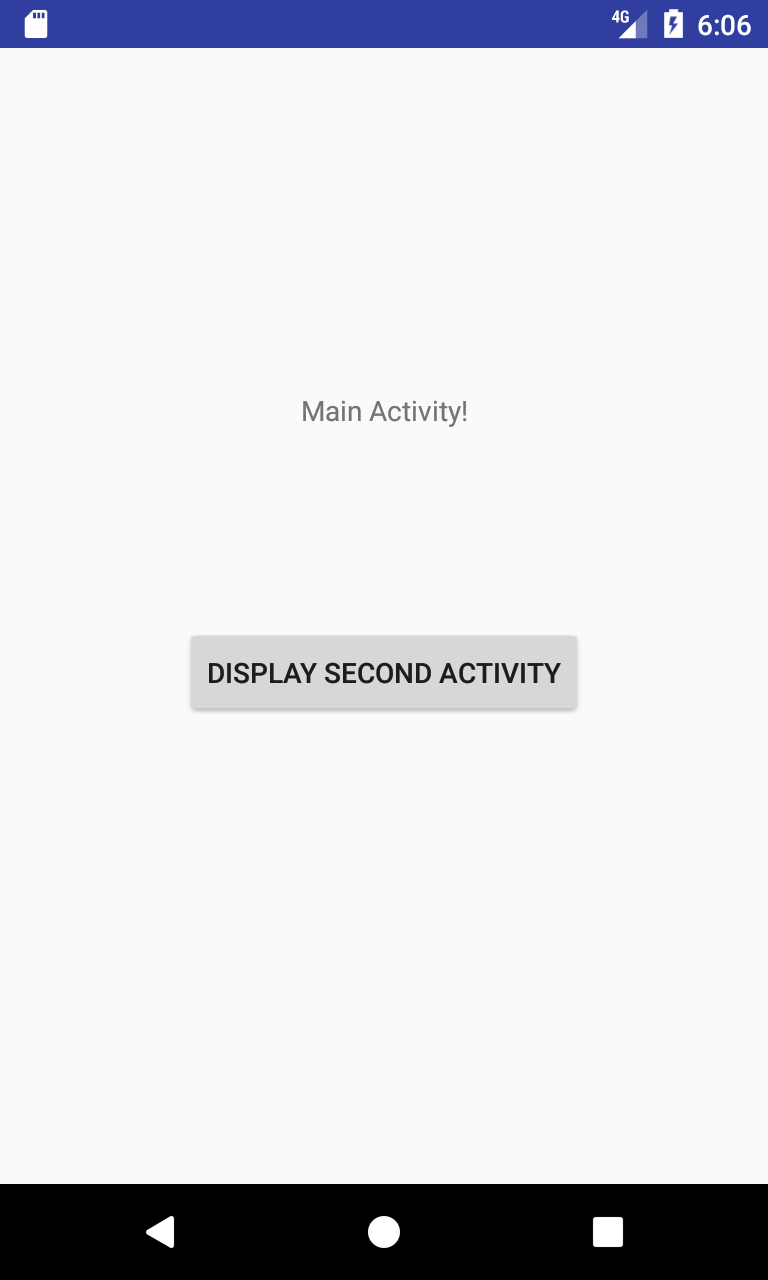
\includegraphics[width=0.7\linewidth]{Screenshot_1496833584}
		\caption{Hasil Akhir (1)}
		\label{fig:screenshot_1496833584}
	\end{minipage}
	\begin{minipage}{.5\textwidth}
		\centering
		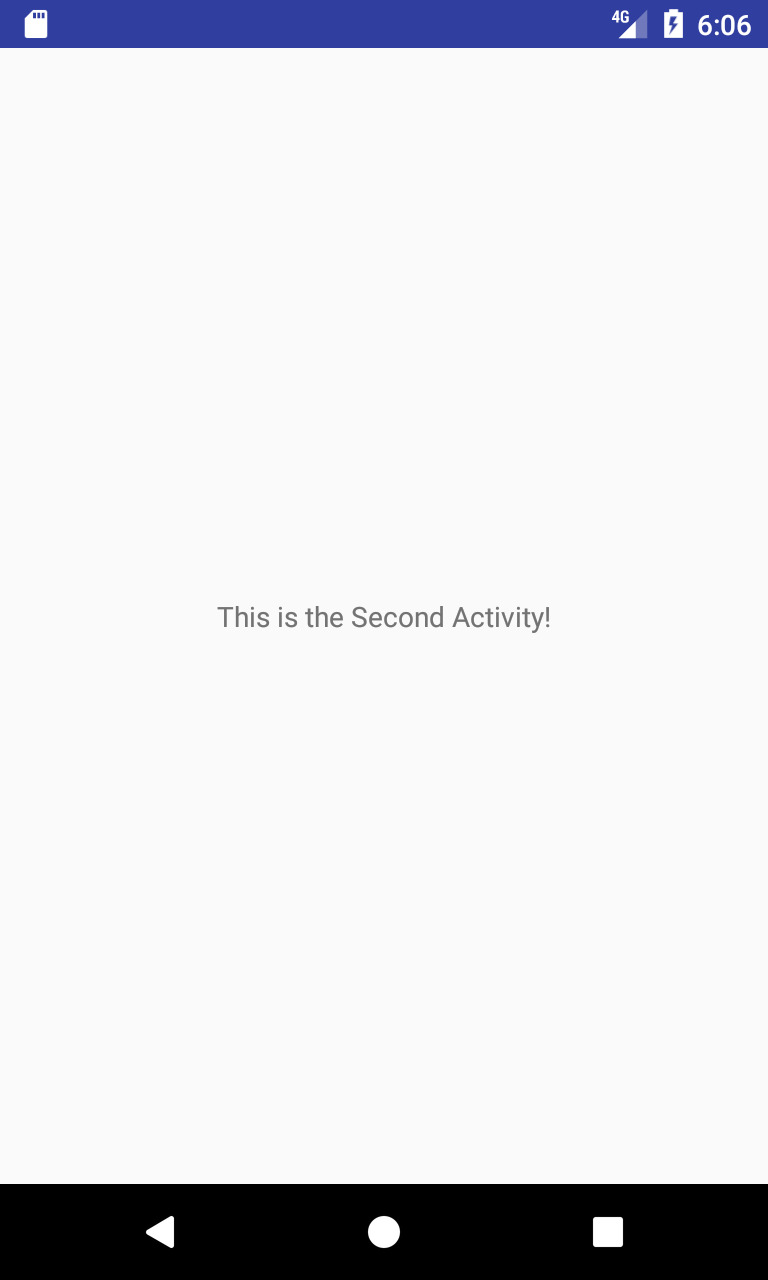
\includegraphics[width=0.7\linewidth]{Screenshot_1496833588}
		\caption{Hasil Akhir (2)}
		\label{fig:screenshot_1496833588}
	\end{minipage}
	\end{figure}
	
\end{enumerate}

\subsection{Mendapatkan Hasil dari \texttt{Activity}}

\begin{enumerate}
	\item Gunakan kembali proyek \textbf{UsingIntent}.
	\item Buka \texttt{activity\_second.xml}, lalu \textit{copy-paste} listing di bawah ini.
	
	\begin{minted}{xml}
	<?xml version="1.0" encoding="utf-8"?>
	<android.support.constraint.ConstraintLayout xmlns:android="http://schemas.android.com/apk/res/android"
		xmlns:app="http://schemas.android.com/apk/res-auto"
		xmlns:tools="http://schemas.android.com/tools"
		android:layout_width="match_parent"
		android:layout_height="match_parent"
		tools:context="com.example.usingintent.SecondActivity">
		
		<TextView
			android:id="@+id/textView2"
			android:layout_width="wrap_content"
			android:layout_height="wrap_content"
			android:text="Please enter your name"
			app:layout_constraintBottom_toBottomOf="parent"
			app:layout_constraintHorizontal_bias="0.067"
			app:layout_constraintLeft_toLeftOf="parent"
			app:layout_constraintRight_toRightOf="parent"
			app:layout_constraintTop_toTopOf="parent"
			app:layout_constraintVertical_bias="0.066"
			tools:layout_constraintBottom_creator="1"
			tools:layout_constraintLeft_creator="1"
			tools:layout_constraintRight_creator="1"
			tools:layout_constraintTop_creator="1" />
		
		<TextView
			android:id="@+id/textView3"
			android:layout_width="wrap_content"
			android:layout_height="wrap_content"
			android:text="This is the Second Activity!"
			app:layout_constraintLeft_toLeftOf="parent"
			app:layout_constraintTop_toTopOf="parent"
			app:layout_constraintBottom_toBottomOf="parent"
			app:layout_constraintRight_toRightOf="parent"
			tools:layout_constraintTop_creator="1"
			tools:layout_constraintRight_creator="1"
			tools:layout_constraintBottom_creator="1"
			tools:layout_constraintLeft_creator="1"
			app:layout_constraintHorizontal_bias="0.073"
			app:layout_constraintVertical_bias="0.032" />
		
		<EditText
			android:id="@+id/editText"
			android:layout_width="wrap_content"
			android:layout_height="wrap_content"
			android:layout_marginLeft="16dp"
			android:layout_marginRight="8dp"
			android:ems="10"
			android:hint="John Doe"
			android:inputType="textPersonName"
			app:layout_constraintBottom_toBottomOf="parent"
			app:layout_constraintHorizontal_bias="0.0"
			app:layout_constraintLeft_toLeftOf="parent"
			app:layout_constraintRight_toRightOf="parent"
			app:layout_constraintTop_toTopOf="parent"
			app:layout_constraintVertical_bias="0.106" />
		
		<Button
			android:id="@+id/button2"
			android:onClick="onClick"
			android:layout_width="wrap_content"
			android:layout_height="wrap_content"
			android:layout_marginLeft="16dp"
			android:text="OK"
			app:layout_constraintLeft_toLeftOf="parent"
			android:layout_marginRight="8dp"
			app:layout_constraintRight_toRightOf="parent"
			app:layout_constraintTop_toTopOf="parent"
			android:layout_marginTop="8dp"
			app:layout_constraintBottom_toBottomOf="parent"
			android:layout_marginBottom="8dp"
			app:layout_constraintHorizontal_bias="0.0"
			app:layout_constraintVertical_bias="0.19" />
	</android.support.constraint.ConstraintLayout>
	\end{minted}
	
	\item Buka file \texttt{SecondActivity.java}, lalu \textit{copy-paste} listing di bawah ini.
	
	\begin{minted}{java}
	package com.example.usingintent;
	
	import android.app.Activity;
	import android.content.Intent;
	import android.net.Uri;
	import android.os.Bundle;
	import android.view.View;
	import android.widget.EditText;
	
	public class SecondActivity extends Activity {
		
		@Override
		protected void onCreate(Bundle savedInstanceState) {
			super.onCreate(savedInstanceState);
			setContentView(R.layout.activity_second);
		}
		
		public void onClick(View view) {
			Intent data = new Intent();
			
			// get the EditText view
			EditText txt_username = (EditText) findViewById(R.id.editText);
			
			// set the data to pass back
			data.setData(Uri.parse(txt_username.getText().toString()));
			setResult(RESULT_OK, data);
			
			// close the activity
			finish();
		}
	}
	\end{minted}
	
	\item Buka file \texttt{MainActivity.java}, lalu \textit{copy-paste} listing di bawah ini.
	\begin{minted}{java}
	package com.example.usingintent;
	
	import android.app.Activity;
	import android.content.Intent;
	import android.os.Bundle;
	import android.view.View;
	import android.widget.Toast;
	
	public class MainActivity extends Activity {
		
		int request_Code = 1;
		
		@Override
		protected void onCreate(Bundle savedInstanceState) {
			super.onCreate(savedInstanceState);
			setContentView(R.layout.activity_main);
		}
		
		public void onClick(View view) {
			startActivityForResult(new Intent("com.example.usingintent.SecondActivity"), request_Code);
		}
		
		public void onActivityResult(int requestCode, int resultCode, Intent data) {
			if (requestCode == request_Code) {
				if (resultCode == RESULT_OK) {
					Toast.makeText(this,data.getData().toString(),
					Toast.LENGTH_SHORT).show();
				}
			}
		}
	}
	\end{minted}
	
	\item Tekan \texttt{Shift+F9} (atau pilih \texttt{Run > Debug}) untuk men-\textit{debug} aplikasi. Pilih salah satu Android Virtual Devices yang kalian inginkan. Hasil akhir ditunjukkan pada Figure \ref{fig:screenshot_1496836379}, Figure \ref{fig:screenshot_1496836388}, Figure \ref{fig:screenshot_1496836393}, dan Figure \ref{fig:screenshot_1496836397}.
	
	\begin{figure}[htbp]
	\begin{minipage}{.5\textwidth}
		\centering
		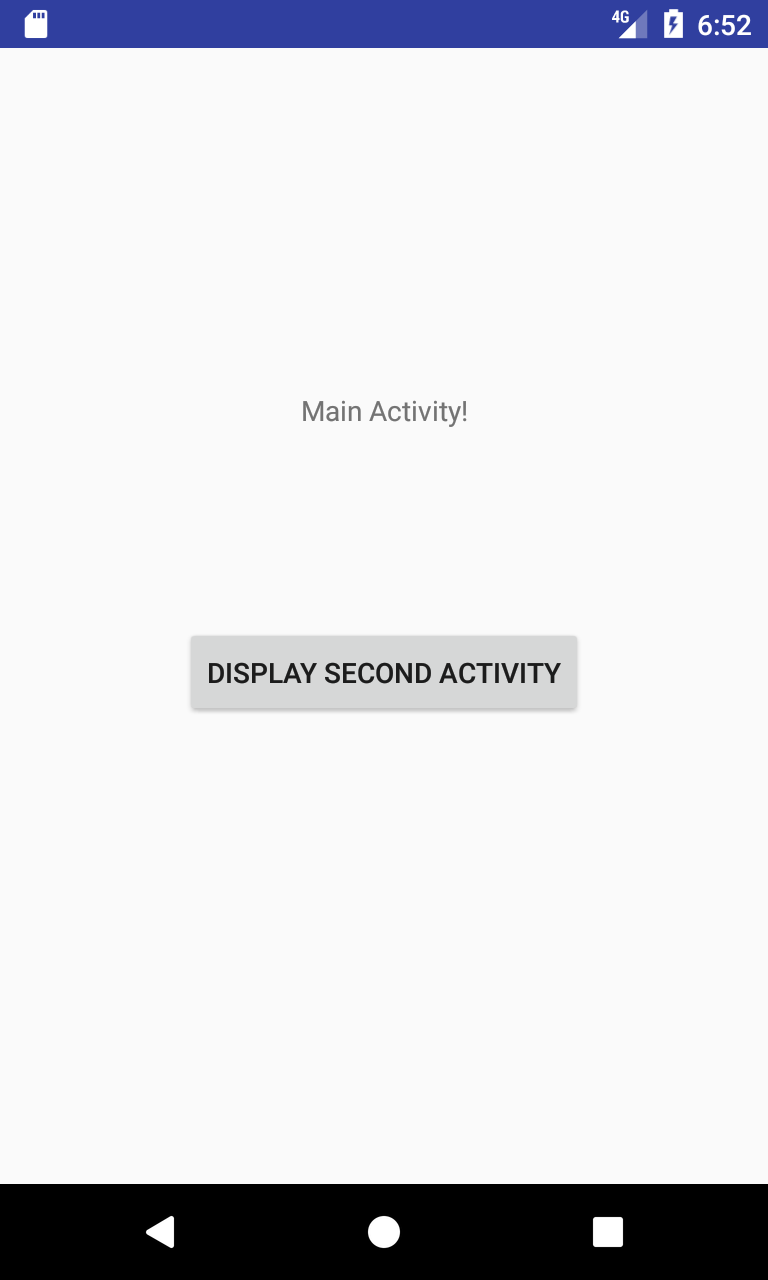
\includegraphics[width=0.7\linewidth]{Screenshot_1496836379}
		\caption{Hasil Akhir (1)}
		\label{fig:screenshot_1496836379}
	\end{minipage}
	\begin{minipage}{.5\textwidth}
		\centering
		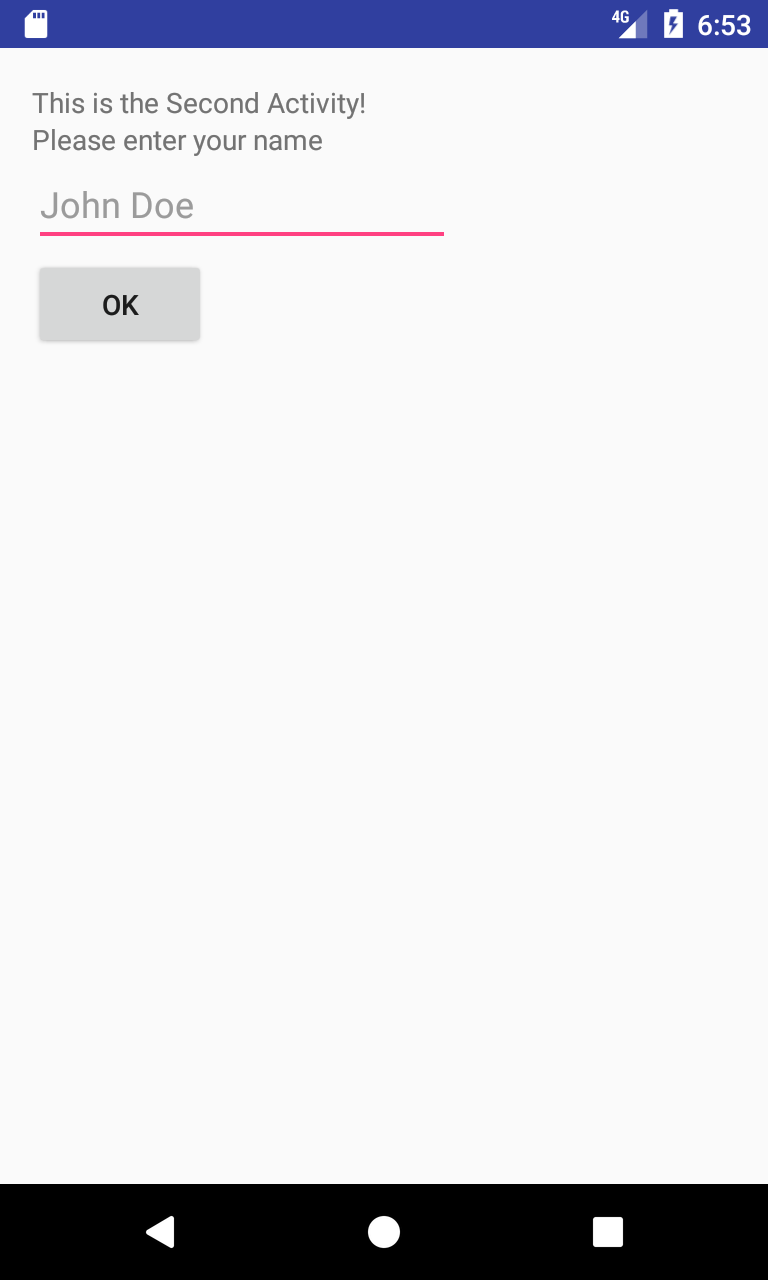
\includegraphics[width=0.7\linewidth]{Screenshot_1496836388}
		\caption{Hasil Akhir (2)}
		\label{fig:screenshot_1496836388}
	\end{minipage}
	\end{figure}

	\begin{figure}[htbp]
		\begin{minipage}{.5\textwidth}
		\centering
		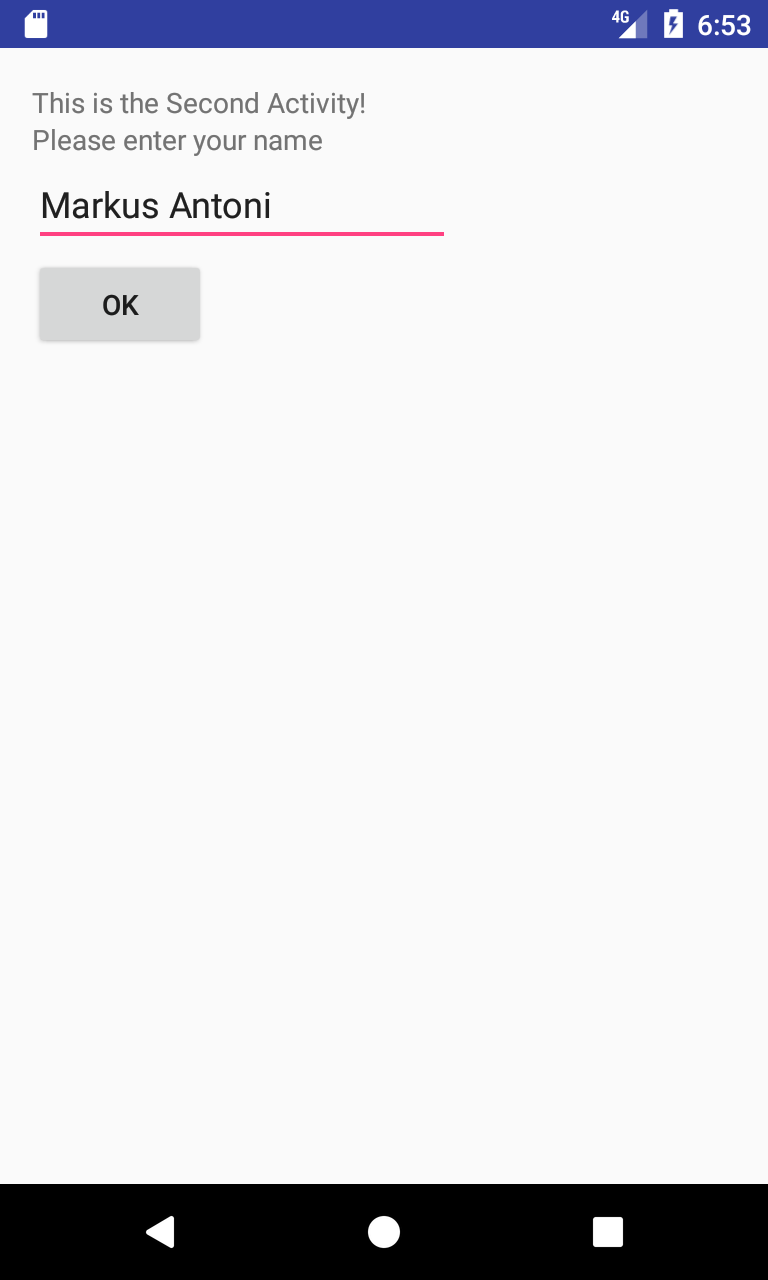
\includegraphics[width=0.7\linewidth]{Screenshot_1496836393}
		\caption{Hasil Akhir (3)}
		\label{fig:screenshot_1496836393}
	\end{minipage}
	\begin{minipage}{.5\textwidth}
		\centering
		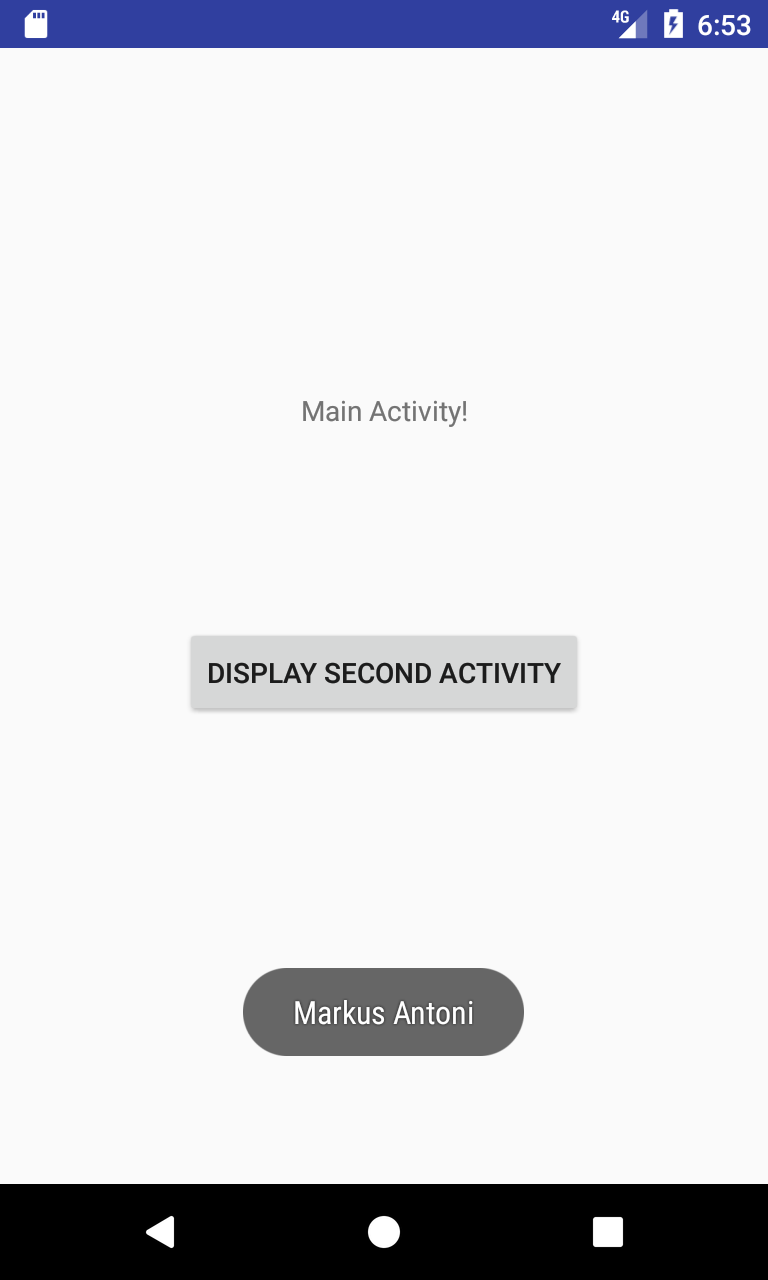
\includegraphics[width=0.7\linewidth]{Screenshot_1496836397}
		\caption{Hasil Akhir (4)}
		\label{fig:screenshot_1496836397}
	\end{minipage}
	\end{figure}

\end{enumerate}

\subsection{Passing Data Menggunakan Obyek Intent}

\begin{enumerate}
	\item Buat proyek baru dengan ketentuan berikut ini.
	\begin{itemize}
		\item Nama aplikasi: \textbf{PassingData}
		\item Pilih \textbf{Empty Activity}
	\end{itemize}

	\item Pilih \texttt{File > New > Activity > Empty Activity}. \texttt{Activity} yang baru tersebut diberi nama \textbf{SecondActivity}.
	
	\item Buka file \texttt{AndroidManifest.xml}, lalu \textit{copy-paste} listing berikut ini.
	
	\begin{minted}{xml}
	<?xml version="1.0" encoding="utf-8"?>
		<manifest xmlns:android="http://schemas.android.com/apk/res/android"
		package="com.example.passingdata">
		
		<application
			android:allowBackup="true"
			android:icon="@mipmap/ic_launcher"
			android:label="@string/app_name"
			android:roundIcon="@mipmap/ic_launcher_round"
			android:supportsRtl="true"
			android:theme="@style/AppTheme">
			<activity android:name=".MainActivity">
				<intent-filter>
					<action android:name="android.intent.action.MAIN" />
					<category android:name="android.intent.category.LAUNCHER" />
				</intent-filter>
			</activity>
			<activity android:name=".SecondActivity">
				<intent-filter>
					<action android:name="com.example.passingdata.SecondActivity" />
					<category android:name="android.intent.category.DEFAULT" />
				</intent-filter>
			</activity>
		</application>
	
	</manifest>
	\end{minted}
	
	\item Buka file \texttt{activity\_main.xml}, lalu \textit{copy-paste} listing berikut ini.
	
	\begin{minted}{xml}
	<?xml version="1.0" encoding="utf-8"?>
	<android.support.constraint.ConstraintLayout xmlns:android="http://schemas.android.com/apk/res/android"
		xmlns:app="http://schemas.android.com/apk/res-auto"
		xmlns:tools="http://schemas.android.com/tools"
		android:layout_width="match_parent"
		android:layout_height="match_parent"
		tools:context="com.example.passingdata.MainActivity">
		
		<Button
			android:layout_width="wrap_content"
			android:layout_height="wrap_content"
			android:text="Click to go to Second Activity"
			android:id="@+id/button"
			android:onClick="onClick"
			app:layout_constraintLeft_toLeftOf="parent"
			app:layout_constraintTop_toTopOf="parent"
			app:layout_constraintBottom_toBottomOf="parent"
			app:layout_constraintRight_toRightOf="parent" />
	
	</android.support.constraint.ConstraintLayout>
	\end{minted}
	
	\item Buka file \texttt{activity\_second.xml}, lalu \textit{copy-paste} listing berikut ini.
	
	\begin{minted}{xml}
	<?xml version="1.0" encoding="utf-8"?>
		<android.support.constraint.ConstraintLayout xmlns:android="http://schemas.android.com/apk/res/android"
		xmlns:app="http://schemas.android.com/apk/res-auto"
		xmlns:tools="http://schemas.android.com/tools"
		android:layout_width="match_parent"
		android:layout_height="match_parent"
		tools:context="com.example.passingdata.SecondActivity">
		
		<TextView
			android:layout_width="wrap_content"
			android:layout_height="wrap_content"
			android:text="Welcome to the Second Activity"
			android:id="@+id/textView"
			app:layout_constraintLeft_toLeftOf="parent"
			app:layout_constraintRight_toRightOf="parent"
			app:layout_constraintTop_toTopOf="parent"
			app:layout_constraintHorizontal_bias="0.529"
			app:layout_constraintBottom_toTopOf="@+id/button" />
		
		<Button
			android:layout_width="wrap_content"
			android:layout_height="wrap_content"
			android:text="Click to go to Main Activity"
			android:id="@+id/button"
			android:onClick="onClick"
			app:layout_constraintLeft_toLeftOf="parent"
			app:layout_constraintBottom_toBottomOf="parent"
			app:layout_constraintRight_toRightOf="parent"
			app:layout_constraintHorizontal_bias="0.536"
			app:layout_constraintTop_toBottomOf="@+id/textView" />
	
	</android.support.constraint.ConstraintLayout>
	
	\end{minted}
	
	\item Buka file \texttt{MainActivity.java}, lalu \textit{copy-paste} listing di bawah ini.
	
	\begin{minted}{java}
	package com.example.passingdata;
	
	import android.content.Intent;
	import android.os.Bundle;
	import android.support.v7.app.AppCompatActivity;
	import android.view.View;
	import android.widget.Toast;
	
	public class MainActivity extends AppCompatActivity {
	
		@Override
		protected void onCreate(Bundle savedInstanceState) {
		super.onCreate(savedInstanceState);
		setContentView(R.layout.activity_main);
		}
		
		public void onClick(View view) {
		
			Intent i = new Intent("com.example.passingdata.SecondActivity");
			
			// use putExtra() to add new name/value pairs
			i.putExtra("str1", "This is a string");
			i.putExtra("age1", 25);
			
			// use a Bundle object to add new name/values pairs
			Bundle extras = new Bundle();
			extras.putString("str2", "This is another string");
			extras.putInt("age2", 35);
			
			// attach the Bundle object to the Intent object
			i.putExtras(extras);
			
			// start the activity to get a result back
			startActivityForResult(i, 1);
		}
		
		public void onActivityResult(int requestCode, int resultCode, Intent data) {
			// check if the request code is 1
			if (requestCode == 1) {
			
				// if the result is OK
				if (resultCode == RESULT_OK) {
				
					// get the result using getIntExtra()
					Toast.makeText(this, Integer.toString(
					data.getIntExtra("age3", 0)),
					Toast.LENGTH_SHORT).show();
					
					// get the result using getData()
					Toast.makeText(this, data.getData().toString(),
					Toast.LENGTH_SHORT).show();
				}
			}
		}
	}
	\end{minted}
	
	\item Buka file \texttt{SecondActivity.java}, lalu \textit{copy-paste} listing di bawah ini.
	
	\begin{minted}{java}
	package com.example.passingdata;
	
	import android.content.Intent;
	import android.net.Uri;
	import android.os.Bundle;
	import android.support.v7.app.AppCompatActivity;
	import android.view.View;
	import android.widget.Toast;
	
	public class SecondActivity extends AppCompatActivity {
	
		@Override
		protected void onCreate(Bundle savedInstanceState) {
			super.onCreate(savedInstanceState);
			setContentView(R.layout.activity_second);
			
			// get the data passed in using getStringExtra()
			Toast.makeText(this,getIntent().getStringExtra("str1"),
			Toast.LENGTH_SHORT).show();
			
			// get the data passed in using getIntExtra()
			Toast.makeText(this,Integer.toString(
			getIntent().getIntExtra("age1", 0)),
			Toast.LENGTH_SHORT).show();
			
			// get the Bundle object passed in
			Bundle bundle = getIntent().getExtras();
			
			// get the data using the getString()
			Toast.makeText(this, bundle.getString("str2"),
			Toast.LENGTH_SHORT).show();
			
			// get the data using the getInt() method
			Toast.makeText(this,Integer.toString(bundle.getInt("age2")),
			Toast.LENGTH_SHORT).show();
		}
		
		public void onClick(View view) {
			// use an Intent object to return data
			
			Intent i = new Intent();
			
			// use the putExtra() method to return some value
			i.putExtra("age3", 45);
			
			// use the setData() method to return some value
			i.setData(Uri.parse("Something passed back to main activity"));
			
			// set the result with OK and the Intent object
			setResult(RESULT_OK, i);
			
			// destroy the current activity
			finish();
		}
	}
	\end{minted}
	
	\item Tekan \texttt{Shift+F9} (atau pilih \texttt{Run > Debug}) untuk men-\textit{debug} aplikasi. Pilih salah satu Android Virtual Devices yang kalian inginkan. Hasil akhir ditunjukkan pada Figure \ref{fig:screenshot_1496841041}, Figure \ref{fig:screenshot_1496841043}, Figure \ref{fig:screenshot_1496841045}, Figure \ref{fig:screenshot_1496841047}, Figure \ref{fig:screenshot_1496841050}, Figure \ref{fig:screenshot_1496841052}, Figure \ref{fig:screenshot_1496841055}, dan Figure \ref{fig:screenshot_1496841057}.
	
	\begin{figure}[htbp]
		\begin{minipage}{.5\textwidth}
			\centering
			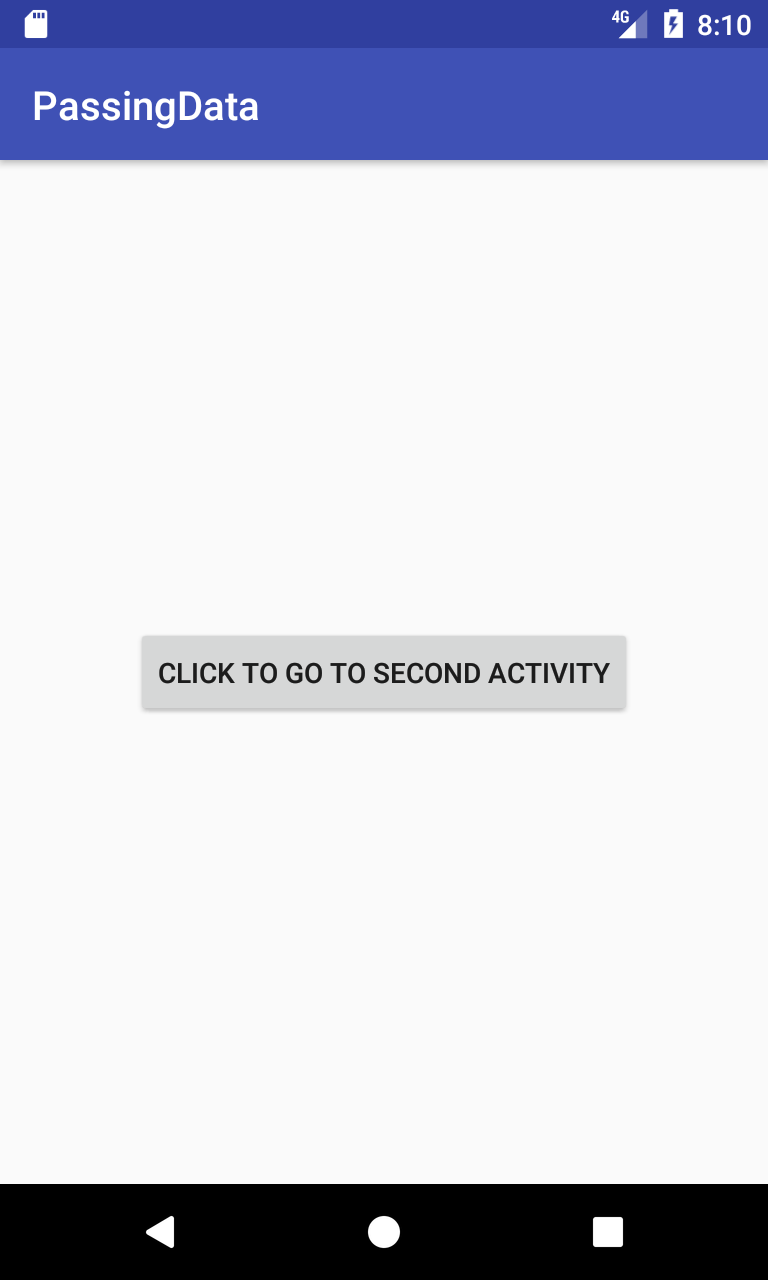
\includegraphics[width=0.7\linewidth]{Screenshot_1496841041}
			\caption{Hasil Akhir (1)}
			\label{fig:screenshot_1496841041}
		\end{minipage}
		\begin{minipage}{.5\textwidth}
			\centering
			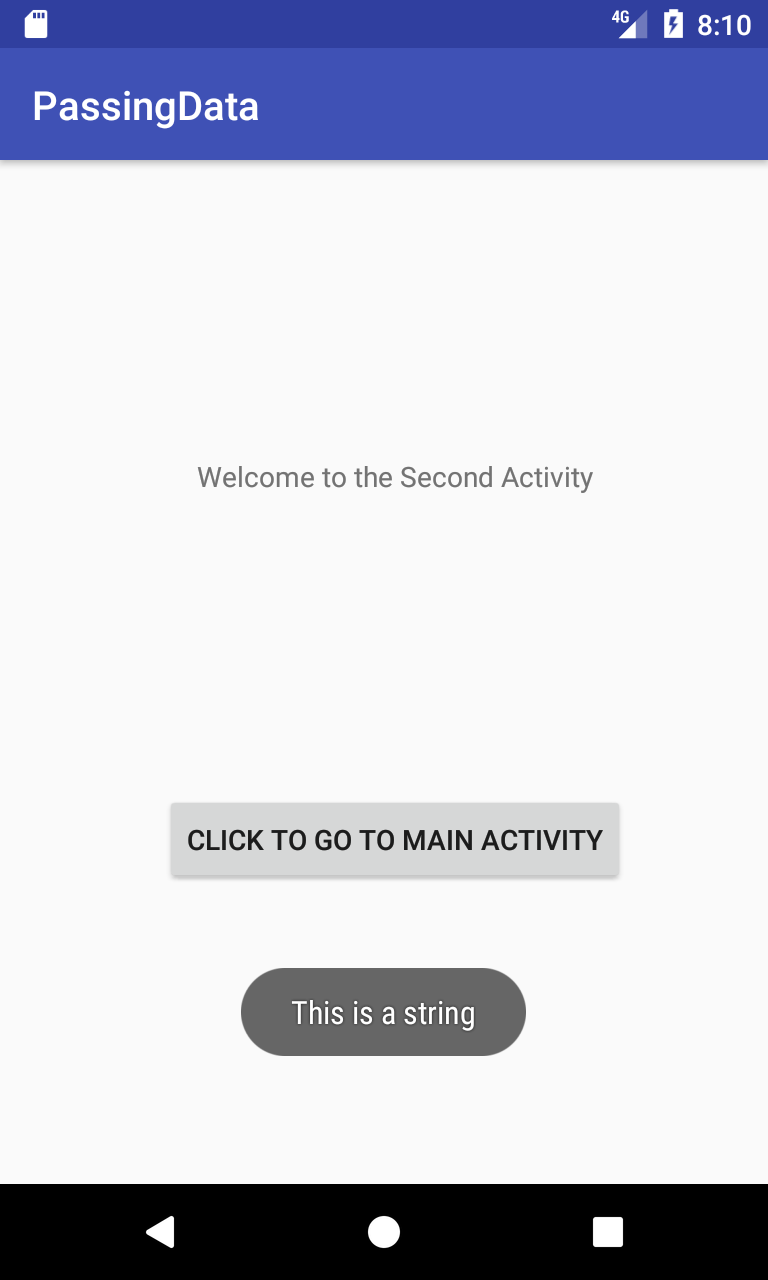
\includegraphics[width=0.7\linewidth]{Screenshot_1496841043}
			\caption{Hasil Akhir (2)}
			\label{fig:screenshot_1496841043}
		\end{minipage}
	\end{figure}

	\begin{figure}[htbp]
		\begin{minipage}{.5\textwidth}
			\centering
			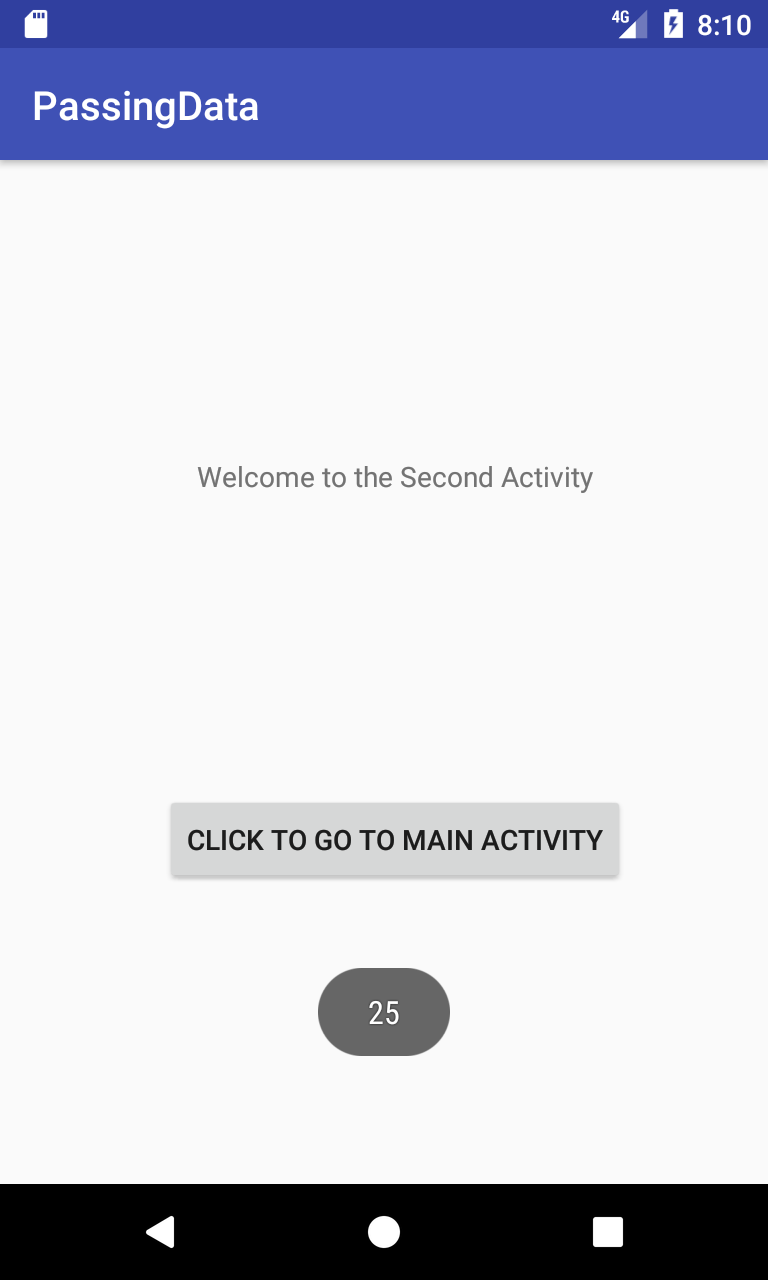
\includegraphics[width=0.7\linewidth]{Screenshot_1496841045}
			\caption{Hasil Akhir (1)}
			\label{fig:screenshot_1496841045}
		\end{minipage}
		\begin{minipage}{.5\textwidth}
			\centering
			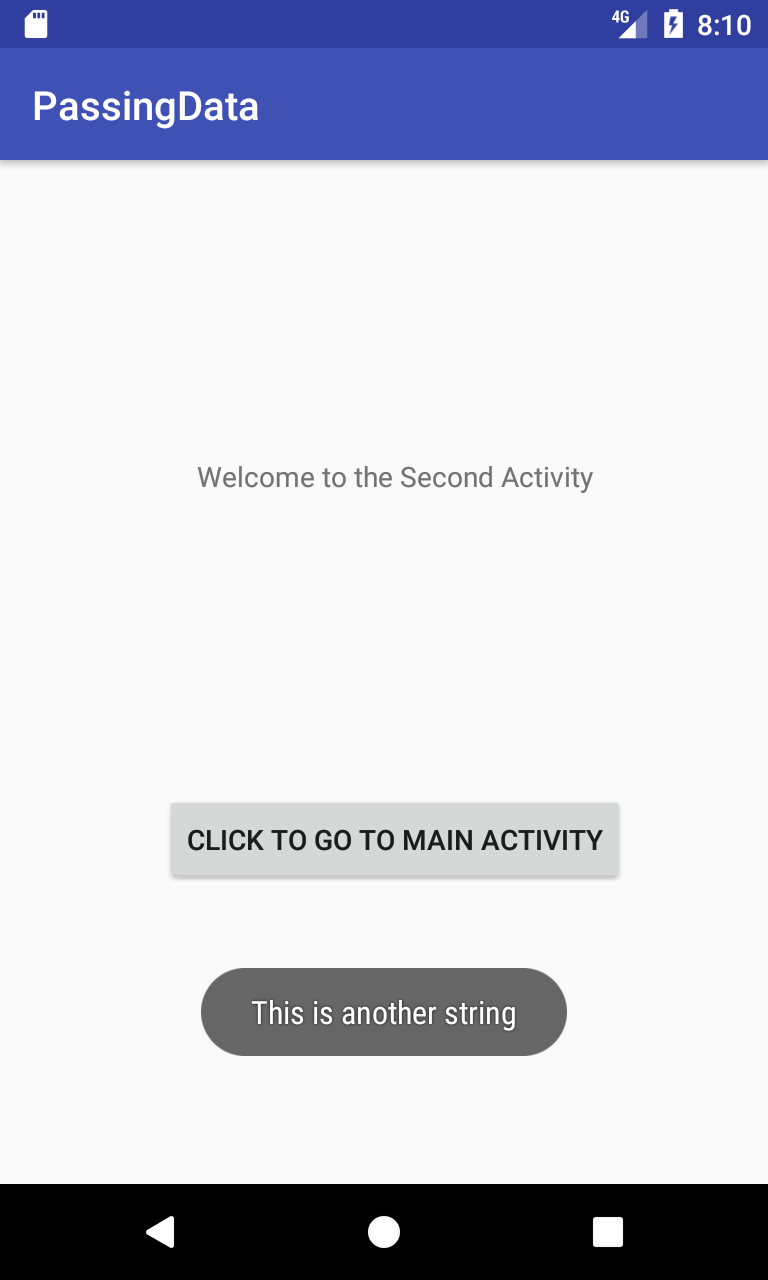
\includegraphics[width=0.7\linewidth]{Screenshot_1496841047}
			\caption{Hasil Akhir (2)}
			\label{fig:screenshot_1496841047}
		\end{minipage}
	\end{figure}

	\begin{figure}[htbp]
		\begin{minipage}{.5\textwidth}
			\centering
			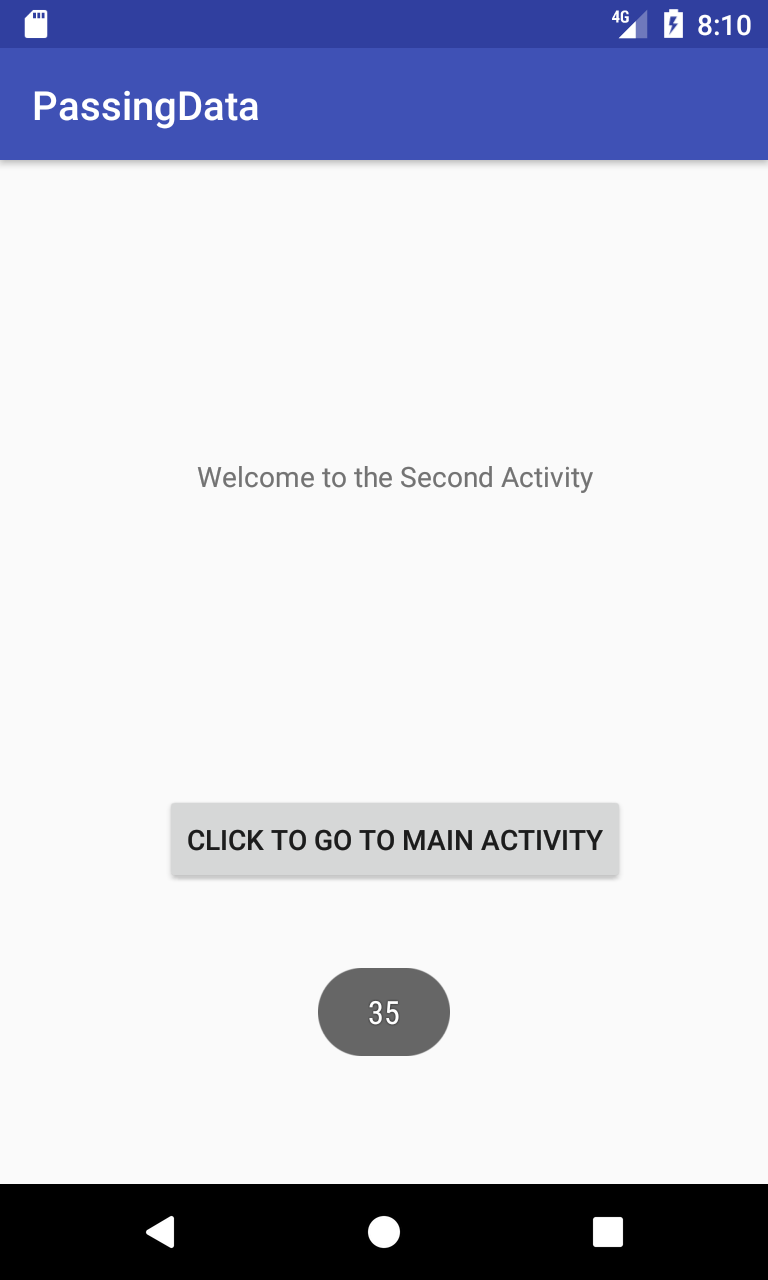
\includegraphics[width=0.7\linewidth]{Screenshot_1496841050}
			\caption{Hasil Akhir (1)}
			\label{fig:screenshot_1496841050}
		\end{minipage}
		\begin{minipage}{.5\textwidth}
			\centering
			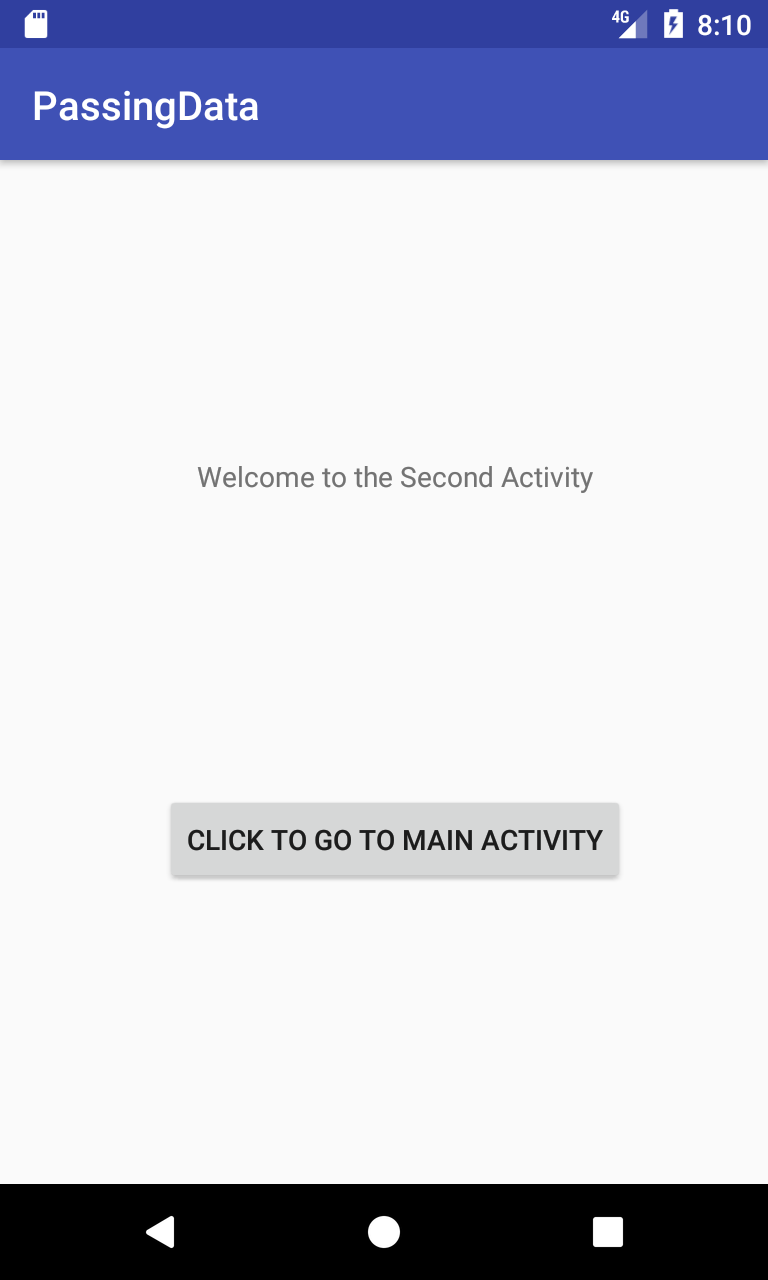
\includegraphics[width=0.7\linewidth]{Screenshot_1496841052}
			\caption{Hasil Akhir (2)}
			\label{fig:screenshot_1496841052}
		\end{minipage}
	\end{figure}

	\begin{figure}[htbp]
		\begin{minipage}{.5\textwidth}
			\centering
			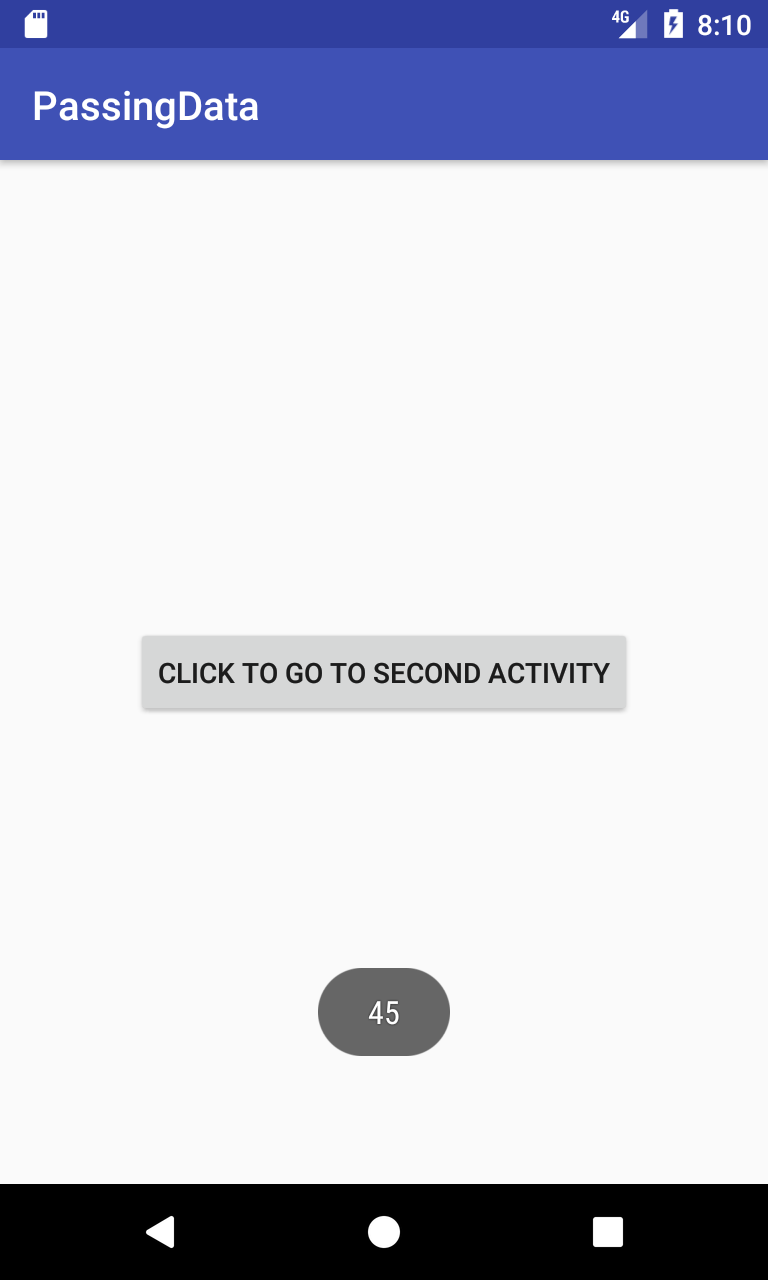
\includegraphics[width=0.7\linewidth]{Screenshot_1496841055}
			\caption{Hasil Akhir (1)}
			\label{fig:screenshot_1496841055}
		\end{minipage}
		\begin{minipage}{.5\textwidth}
			\centering
			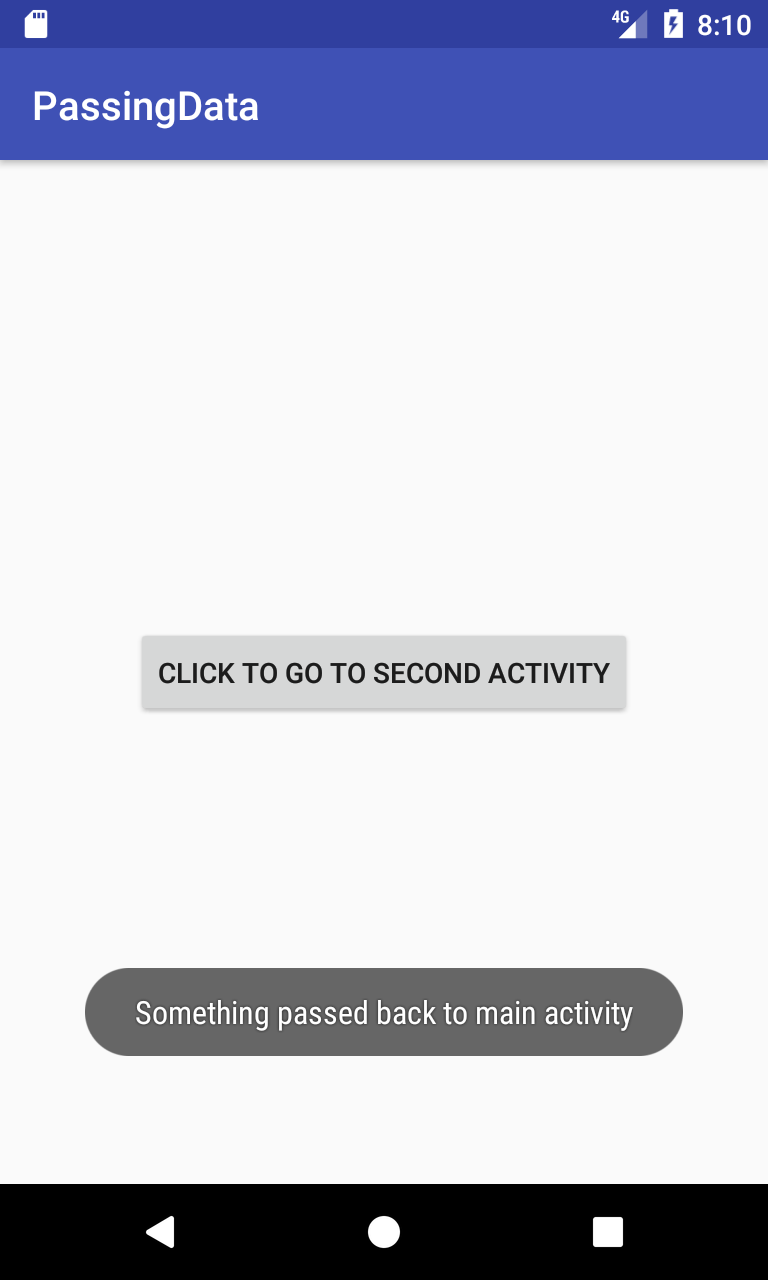
\includegraphics[width=0.7\linewidth]{Screenshot_1496841057}
			\caption{Hasil Akhir (2)}
			\label{fig:screenshot_1496841057}
		\end{minipage}
	\end{figure}
	
\end{enumerate}
\vspace*{\fill}
\begin{center}
\large{\textbf{THE END}}
\end{center}

\end{document}